\label{texfile:GWF}
Currently, every \mfus\ model must contain a \gwf\ domain, which may be reduced to a single layer of very low hydraulic conductivity in cases where \gwf\ flow and interaction with other model domains is to be neglected.

\subsection{Generating a Layered \gwf\ Domain}
A \mfus\ 3D groundwater flow (\gwf) domain can be generated from the template using this instruction:

\ins{generate layered gwf domain}
    {This subtask has instructions that are used to define:
     \begin{itemize}
        \item Element zone numbering scheme
        \item Top elevation (i.e. $z$-coordinate)
        \item Mesh layers and vertical discretization
    \end{itemize}

    Subtask instructions will be read and processed until an \textsf{end} instruction is encountered.  We suggest appending the subtask name to the \textsf{end} instruction:

    {\Large \sf end generate layered gwf domain}
    }

The construction of the 3D \gwf\ finite-element mesh proceeds from top to bottom.  First, we define the top elevation, then add layers one at a time until we reach the base of the domain. By default, element zone numbers will be assigned by layer number.  If the template mesh is divided into horizontal patches with unique zone numbers, these can be assigned instead to the 3D GWF mesh \footnote{The verification example \texttt{MUT\_Examples$\backslash$6\_Abdul\_Prism\_Cell} uses this option to define \swf\ domain zones.} using this instruction:

\ins{Zone by template}
    {Causes \mut\ to assign the template mesh element zone number to the corresponding 3D \gwf\ element.

    {\em This instruction should appear in the input file at the beginning of the \textsf{generate layered gwf domain} subtask before new layers are added.}
    }

\subsubsection{Defining the Top Elevation} \label{section:topelev}
To assign an elevation to the top layer of template nodes use this instruction:

\ins{top elevation}
    {This subtask defines the elevation (i.e. $z$-coordinate) of the top layer of nodes in the \gwf\ finite-element template mesh in one of these ways:
     \begin{itemize}
        \item By assigning a given elevation to all nodes
        \item By reading variable elevation data from a file
        \item By interpolating elevation data from a function $z(x)$ where the elevation $z$ varies by the nodes $x$ coordinate.
     \end{itemize}
     Once the elevation is defined, an \textsf{end} instruction is required to stop the subtask e.g.\:

    {\Large \sf end top elevation}
    }

 The top elevation can be defined by one of these instructions: \label{'Page:TopElev'}

 \ins{elevation constant}
    {\squish
    \begin{enumerate}
    \item \rnum{elev}\  The elevation \rnum{elev}\ will be assigned to all top layer nodes.
    \end{enumerate}
    \squish
    }

 \ins{elevation from gb file}
    {\squish
    \begin{enumerate}
    \item \str{file}\  The elevation data in the \gb\ nodal property file named \str{file}\ will be assigned to the top layer nodes.
    \end{enumerate}
    \squish
    }

The \gb\ nodal property file uses a legacy binary file format. You can develop your own ascii input files and read them using this instruction:

 \ins{elevation from list file}
    {\squish
    \begin{enumerate}
    \item \str{file}\  The elevation data in the ascii file named  \str{file}\ will be assigned to the top layer nodes.
    \end{enumerate}
    \squish
    }

Part of a sample list file \footnote{The verification example \texttt{MUT\_Examples$\backslash$6\_Abdul\_MODHMS} uses an ascii file input to define nodal elevations.} is shown here:
    \begin{verbatim}
    Kriged cell top elevation for layer 1
     4.414571762E+000
     4.415914536E+000
     ...
     4.415914536E+000
     \end{verbatim}
     \squish
Some key features of this example are:
\begin{itemize}
  \item The first line of the file is discarded, and in this case contains a string describing the data.
  \item You must supply a value for each node in the template finite-element mesh.
  \item The data is read in free format so there can be more than one value entered per line.
  \item Only the start and end of the file are shown here, with the string '\texttt{...}' replacing the middle portion.
\end{itemize}

To define the top elevation as a function of $x$ (usually used for cross-sectional models) use this instruction:

 \ins{elevation from xz pairs}
    {
    \squish
    \begin{enumerate}
    \item \rnum{x(1)}, \rnum{y(1)}  First $x, z$ coordinate pair.
    \item \textbf{...}
    \item \rnum{x(n)}, \rnum{y(n)}  nth $x, z$ coordinate pair.
    \end{enumerate}

     An elevation is calculated for each chosen cell, based on it's $x$-coordinate location, by interpolating an elevation from the given list of  $xz$-coordinate pairs.

     This subtask reads a list of $xz$-coordinate pairs until an \textsf{end} instruction is encountered e.g.\:

    {\Large \sf end elevation from xz pairs}
    }

Here is an example showing the use of this instruction \footnote{The verification example \texttt{MUT\_Examples$\backslash$1\_VSF\_Hillslope} uses the \textsf{elevation from xz pairs} pairs instruction to define the top elevation of the cross-sectional domain.}:
    \begin{verbatim}
    elevation from xz pairs
           0.0, 0.0
        1000.0, 100.0
    end elevation from xz pairs
     \end{verbatim}
     \squish
Some key features of this example are:
\begin{itemize}
  \item The two given $xz$ pairs define a line that slopes from $z=0$ at $x=0$ to $z=100.0$ at $x=1000$.  You may supply as many pairs as needed to define the top of your cross-section.
  \item $x$ coordinates must increase continuously from the top of the list to the bottom.
  \item the $x$-range of the supplied pairs should cover the entire $x$-range of the template mesh.
  \item For each node in the template mesh, the $x$ coordinate is used to interpolate an elevation (i.e. $z$ value) using the appropriate $xz$ pair.
\end{itemize}

\subsubsection{Adding Layers} \index{\gwf\ Domain ! layering}
    {\em NOTE: The term layers used here should not be confused with the \mf\ term of the same name. A \mf\ layer is one cell thick, while a \mut\ layer can be one or more elements thick.}

A \mfus\ model must contain at least 1 layer, and each layer is defined using this instruction:     {\index{Grid generation ! \gwf\ Domain ! New layer}

\ins{new layer}
    {This subtask adds a new layer to the \gwf\ domain by defining the layer:
     \begin{itemize}
       \item Base elevation
       \item Vertical discretization
     \end{itemize}

     It reads instructions until an \textsf{end} instruction is found e.g.\:

    {\Large \sf end new layer}
    }

The base elevation is defined using the elevation instructions  described on page~\pageref{'Page:TopElev'} that are given for the \textsf{top elevation} instruction.

By default, a new layer will be assigned the name '\texttt{Layer {\em n}}' where {\em n} is the current layer number.  If you want to assign your own layer name use this instruction:

\ins{Layer name}
    {
    \squish
    \begin{enumerate}
    \item \str{layer\_name} Layer name.
    \end{enumerate}
    \squish
    }

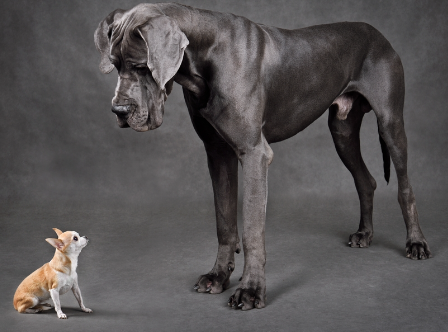
\includegraphics[width=.15\textwidth]{ModelDevelopment} \textit{These names are not currently used in Tecplot output but could/should? be used to create the customlables for zone naming.}



By default, \mut\ will stop and issue a warning message if the computed layer base elevation is greater than or equal to the current layer top elevation.  This instruction forces the base to be below the top by a set amount:

\ins{Minimum layer thickness}
    {\squish
    \begin{enumerate}
    \item \rnum{MinThick} Minumum thickness value[L].
    \end{enumerate}
    This instruction causes \mut\ to enforce a minimum thickness constraint for the current layer. At nodes where the computed layer base elevation is greater than or equal to the current top elevation, \rnum{MinThick} will
    be subtracted from the current top elevation to get the base elevation.
    }

By default, a new layer will not be subdivided vertically unless one the following two instructions is issued.
The first creates a uniform subdivision:

\ins{Uniform sublayering}
    {\squish
    \begin{enumerate}
    \item \inum{nsublayer} Number of sublayers.
    \end{enumerate}
    This instruction divides the layer vertically into \inum{nsublayer}
    elements, which will each have the same element height, equal to the top elevation
    minus the current base elevation divided by \inum{nsublayer}.
    }

This instruction creates a non-uniform subdivision:

\ins{Proportional sublayering}
    {\squish
    \begin{enumerate}
        \item \inum{nsublayer}  Number of proportional sublayers.
        \item \rnum{sub\_thick(i),i=1,\inum{nsublayer}} Proportional thicknesses in order from top to bottom.
    \end{enumerate}
    This instruction can be used if you want to refine the \gwf\ domain mesh vertically,
    for example, in the active zone with the \swf\ domain the ground surface in the .

    It is important to understand that the variable \rnum{sub\_thick} is not
    a true thickness, but is instead a relative thickness, which is used along
    with the layer thickness to determine the element heights in the current
    column.

}

    For example, these instructions:
    \texttt{
            \begin{tabbing}
            AAA\=AAA\=AAA   \kill
                \>Proportional sublayering   \\
                \>   \> 3                     \\
                \>   \> 0.1           \\
                \>   \>1.0            \\
                \>   \>  10.0       \\
                \> end       \\
            \end{tabbing}
    }
    \squish
would subdivide the current layer vertically into three elements, between
    the current base and top elevation, with element height proportions of .1,
    1 and 10 from top to bottom.

This instruction is most often used to define a layer of uniform thickness relative to an uneven top elevation:

\ins{Offset base}
    {\squish
    \begin{enumerate}
    \item \rnum{value} Thickness value (L) by which to offset the layer base elevation.
    \end{enumerate}
    This instruction causes the elevation of the base of the layer to be offset vertically by the given value.  This
    can be used to create a surface a given distance below another surface.
}

    For example, these instructions:
\begin{verbatim}
        top elevation
            elevation from list file
            elev.list
        end top elevation

        new layer
            uniform sublayering
            3

            elevation from list file
            elev.list

            offset base
            -1.0

        end new layer

    end generate layered gwf domain
\end{verbatim}
 create a layer with a top elevation 1 metre below the elevation defined in the raster file \texttt{elev.list}:


\includegraphics[width=.15\textwidth]{UnderConstruction} \textit{Need to check sign on \textsf{offset base} input}

\subsubsection{Cell Connection Properties}  \index{\gwf\ Domain ! cell connection properties}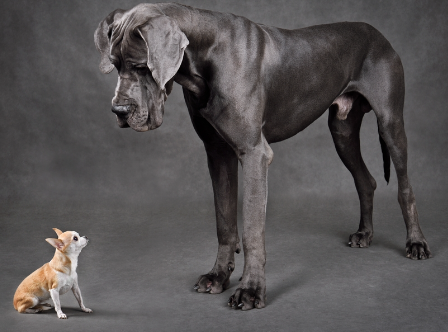
\includegraphics[width=.15\textwidth]{ModelDevelopment} \textit{
\gwf\ cell to \gwf\ cell connection properties are automatically defined by \mut\ based on control-volume approach and element type. The code needs to be checked, verified and documented more completely.}



\subsubsection{Assigning Material Properties}  \index{\gwf\ Domain ! material properties}

\gwf\ domain material properties may vary on a cell-by-cell  basis.  \mut\ offers some simple instructions for selecting cells and assigning material property values to them.  As you might imagine, this instruction:

\ins{choose all cells}
    {Select all cells in the active model domain.
     }

selects all cells in the {\em active} model domain.

This is an example of what we refer to as a {\em generic} instruction, which means it can be applied to any of the currently available model domains: \gwf, \swf\ or \cln.

If our intention is to choose all cells in the \gwf\ domain, we first need to activate it using this instruction:

\ins{active domain}
    {
        \squish
        \begin{enumerate}
        \item \str{Domain}  The name of the domain to be activated: \gwf, \swf\ or \cln\
        \end{enumerate}
        This instruction activates the given domain named in  \str{Domain} so that it will be used with generic instructions such as \textsf{choose all cells}.
    }

So to activate the \gwf\ domain, we would insert these instructions in the input file:
\begin{verbatim}
    active domain
    gwf
\end{verbatim}

These instructions can be used to choose cells in various ways\label{page:cellSelect}:

\ins{choose cell at xyz}
    {
        \squish
        \begin{enumerate}
        \item \rnum{x1}, \rnum{y1}, \rnum{z1}  An $xyz$ coordinate triplet.
        \end{enumerate}
        The cell closest to the given $xyz$ coordinate triplet will be chosen.
    }

\ins{choose cells by layer}
    {
        \squish
        \begin{enumerate}
        \item \inum{layer}  The number of the layer to be chosen.
        \end{enumerate}
        The cells in Modflow layer number \inum{Layer} will be chosen.  Remember that Modflow layers are one cell high and are numbered from the top to the bottom of the model domain.\footnote{ See the verification example \texttt{MUT\_Examples$\backslash$1\_VSF\_Column} which uses the previous two instructions to define a constant head at  the base  and a recharge boundary condition at the top of the 1D column.}
    }

\ins{choose cells from file}
    {
        \squish
        \begin{enumerate}
        \item \str{file}  The file \str{file} containing a list of cell numbers.
        \end{enumerate}
        The cells listed in the file \str{file} will be chosen.  \footnote{ See the verification example \texttt{MUT\_Examples$\backslash$1\_Abdul\_MODHMS} which uses this instruction to assign some cells as inactive.}
    }

\pagebreak
\ins{choose cells from gb elements}
    {
        \squish
        \begin{enumerate}
        \item \str{file}  The \gb\ chosen element file \str{file} containing information concerning the status, chosen or not chosen, of each element in the \gb\ model domain.
        \end{enumerate}
          If an element is flagged as chosen in the \gb\ model domain then the corresponding cell will be chosen in the \mfus\ model domain.  \footnote{ See the verification example \texttt{MUT\_Examples$\backslash$1\_Abdul\_Prism\_Cell} which uses this instruction to assign some cells as inactive.}
    }

\ins{choose cells from gb nodes}
    {
        \squish
        \begin{enumerate}
        \item \str{file}  The \gb\ chosen node \str{file} containing information concerning the status, chosen or not chosen, of each node in the \gb\ model domain.
        \end{enumerate}
          If a node is flagged as chosen in the \gb\ model domain then the corresponding cell will be chosen in the \mfus\ model domain.  \footnote{ See the verification example \texttt{MUT\_Examples$\backslash$1\_Abdul\_Prism\_Cell\_nc} which uses this instruction to assign some cells as inactive.}
    }

The previous two instructions are used to choose cells for the mesh-centered and node-centered approaches respectively.

Cell selection instructions are cumulative.  For example, you can modify the current selection by repeating instructions like  \textsf{choose cell at xyz} or \textsf{choose cells by layer} with different inputs and then assign properties to the current selection.  This instruction clears the selection before beginning new cell selection(s):

\ins{clear chosen cells}
    {Clears the current cell selection.
     }

It is good practice to clear the selection before starting a new selection. \mut\ echoes the results of the selection instructions to the screen and \texttt{.eco} file as shown in this example:
\begin{verbatim}
    clear chosen cells
    	GWF Cells chosen:          0

    choose all cells
    	GWF Cells chosen:      39765
\end{verbatim}
If a cell selection instruction has unexpected results these are good places to check.

\pagebreak
These instructions can be used to assign material properties to the current cell selection:

\ins{gwf kh}
    {
        \squish
        \begin{enumerate}
        \item \rnum{val}  Horizontal hydraulic conductivity [$L$   $T^{-1}$].
        \end{enumerate}
          A horizontal hydraulic conductivity of \rnum{val} is assigned to the chosen cells.
    }


\ins{gwf kv}
    {
        \squish
        \begin{enumerate}
        \item \rnum{val}  Vertical hydraulic conductivity [$L$   $T^{-1}$].
        \end{enumerate}
          A vertical hydraulic conductivity of \rnum{val} is assigned to the chosen cells.
    }

\ins{gwf ss}
    {
        \squish
        \begin{enumerate}
        \item \rnum{val}  Specific storage [$L^{-1}$].
        \end{enumerate}
          A specific storage of \rnum{val} is assigned to the chosen cells.
    }

\ins{gwf sy}
    {
        \squish
        \begin{enumerate}
        \item \rnum{val}  Specific yield (-).
        \end{enumerate}
          A specific yield of  \rnum{val} is assigned to the chosen cells.
    }

\ins{gwf alpha}
    {
        \squish
        \begin{enumerate}
        \item \rnum{val}  Van Genuchten/Brooks-Corey Alpha [$L^{-1}$].
        \end{enumerate}
          A Van Genuchten/Brooks-Corey Alpha of \rnum{val} is assigned to the chosen cells.
    }

\ins{gwf beta}
    {
        \squish
        \begin{enumerate}
        \item \rnum{val}  Specific yield (-).
        \end{enumerate}
          A specific yield of \rnum{val} is assigned to the chosen cells.
    }

\ins{gwf sr}
    {
        \squish
        \begin{enumerate}
        \item \rnum{val}  Residual saturation [-].
        \end{enumerate}
          A residual saturation of \rnum{val} is assigned to the chosen cells.
    }

\ins{gwf brooks}
    {
        \squish
        \begin{enumerate}
        \item \rnum{val}  Brooks-Corey exponent.
        \end{enumerate}
          A Brooks-Corey exponent of \rnum{val} is assigned to the chosen cells.
    }

Defining each different material property as described above can be tedious.  A lookup table of \gwf\ material properties  is provided in the file \texttt{qryGWFMaterials.txt}, located in the \bin\ directory as outlined on page~\pageref{page:userbin}.

In order for \mut\ to access the lookup table, you first need to provide a link to this file using the instruction:

\ins{gwf materials database}
    {
        \squish
        \begin{enumerate}
        \item \str{file}  \gwf\ material properties lookup table file name.
        \end{enumerate}
          \mut\ uses the file \str{file} to look up \gwf\ material properties.
    }

You can now assign a full set of \gwf\ material properties to the current cell selection, as described on page~\pageref{page:cellSelect}, using this instruction:

\ins{chosen cells use gwf material number}
    {
        \squish
        \begin{enumerate}
        \item \inum{val}  \gwf\ material ID number.
        \end{enumerate}
          A unique set of \gwf\ material properties is retrieved from a lookup table, using the given  material ID number \inum{val}, and assigned to the chosen cells.
    }

You can find detailed information about how to use \dbase\ to modify or define your own lookup tables in Tutorial~\ref{tecfile:DbaseUseage}.

\pagebreak
During the model build, each \gwf\ cell is assigned a zone number from either the layer number or 2D template zone number. Just like individual cells, zones can be selected using these instructions\label{page:zoneSelect}:

\ins{choose all zones}
    {Select all zones in the active model domain.
     }

\ins{choose zone number}
    {
        \squish
        \begin{enumerate}
        \item \inum{value}  The number of the zone to be chosen.
        \end{enumerate}
        \squish
    }

\ins{clear chosen zones}
    {Clears the current zone selection.
     }

The zone selection can be converted into a cell selection using this instruction:

\ins{choose cells by chosen zones}
    {If a zone is currently chosen, any cell which has that zone number will be chosen.
     }
This cell selection can now be used to assign material properties.

Below is an example \footnote{See verification example \texttt{MUT\_Examples$\backslash$6\_Abdul\_Prism\_Cell}} of a case in which the element zone numbers have been assigned by layer number for a 3-layer case:

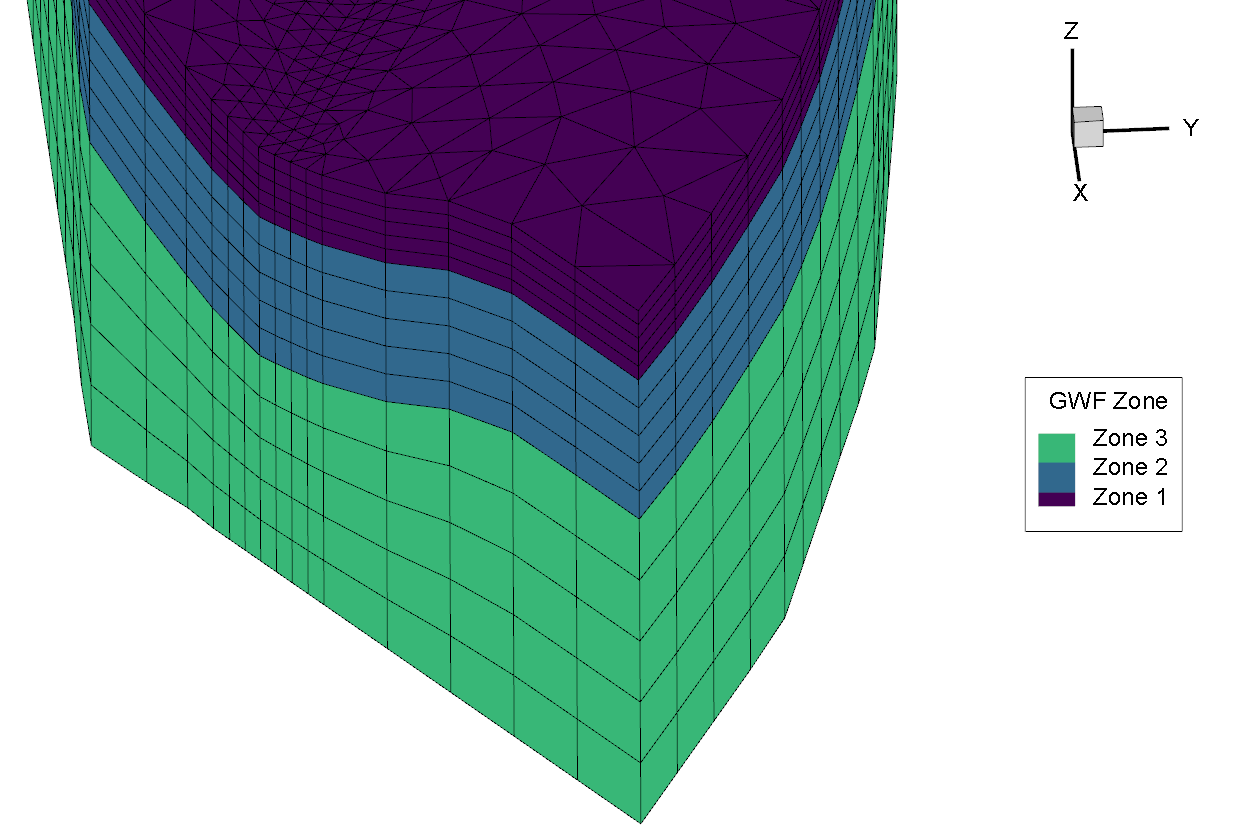
\includegraphics[width=.86\textwidth]{3_10_GWFZones}

\pagebreak
Some key features to note are:
\begin{itemize}
    \item There are 3 zones, corresponding to the layers 1 to 3.
    \item 'Zone 1', coloured dark blue, corresponds to layer 1.  Recall that the \mfus\ mesh is generated from the top down, so layer 1 is at the top of the model domain.
    \item Each layer is composed of multiple \mf\ layers, which are each one cell thick.
\end{itemize}

The following example uses the materials database and zone selection to assign material properties for the 3-layer case:

\begin{verbatim}
    gwf materials database
    	Materials file C:\MUT\MUT_Examples-main\_MUT_USERBIN\qryGWFMaterials.txt

    active domain
    	gwf

    clear chosen zones
    	GWF Zones chosen:          0

    choose zone number
    	Adding zone number:        1
    	GWF zone numbers currently chosen:
    	    1

    choose zone number
    	Adding zone number:        2
    	GWF zone numbers currently chosen:
    	    1
    	    2

    choose zone number
    	Adding zone number:        3
    	GWF zone numbers currently chosen:
    	    1
    	    2
    	    3

    clear chosen cells
    	GWF Cells chosen:          0

    choose cells by chosen zones
    	GWF Cells chosen:      39765

    chosen cells use gwf material number
    	Assigning all chosen GWF cells properties of material               4, Borden sand
    	Kh_Kx:                 1.00000E-05
    	Kv_Kz:                 1.00000E-05
    	Specific Storage:      1.20000E-07
    	Specific Yield:        0.34000
    	Alpha:                  1.9000
    	Beta:                   6.0000
    	Sr:                    0.18000
    	Unsaturated Function Type:   Van Genuchten
\end{verbatim}

Some key features to note are:
\begin{itemize}
    \item As we choose zone numbers, the list of currently chosen zones grows accordingly.
    \item The final number of \gwf\ cells chosen is equal to the total number of cells in the domain, since we had selected all 3 layers prior to converting the  zone selection to a cell selection.
    \item After assignment, the \gwf\ material number, name and assigned property values are echoed to screen and \texttt{.eco} file.
\end{itemize}

\subsubsection{Initial Conditions}  \index{\gwf\ Domain ! initial condition ! initial (starting) head}
An initial (or starting) head should be assigned to each cell in the \gwf\ domain.  This could be an initial guess at the beginning of a transient stress period or a set of hydraulic heads from a previous run.

To assign a uniform hydraulic head to the \gwf\ model domain, you must first make a cell selection as described on page~\pageref{page:cellSelect}, then use this instruction:

\ins{gwf initial head}
    {
        \squish
        \begin{enumerate}
        \item \rnum{value}  Initial (or starting) hydraulic head [L].
        \end{enumerate}
          An initial hydraulic head  of \rnum{value} is assigned to the chosen cells.
    }

To assign a linearly varying head that is a function of $z$ (i.e.\ depth or elevation), use this instruction:
\ins{gwf initial head function of z}
    {
    \squish
    \begin{enumerate}
    \item \rnum{z(1)}, \rnum{head(1)}  First $z, head$ pair.
    \item \rnum{z(2)}, \rnum{head(2)}  Second $z, head$ pair.
    \item \textbf{...}
    \item \rnum{z(n)}, \rnum{head(n)}  nth $z, head$  pair.
    \end{enumerate}

     An initial head is calculated for each chosen cell, based on it's $z$-coordinate location, by interpolating a head from the given list of  $z, head$ pairs.

     This subtask reads a list of $z, head$ pairs until an \textsf{end} instruction is encountered e.g.\:

    {\Large \sf end gwf initial head function of z}
    }

This is commonly used to generate an initial head for a simple column model \footnote{The verification example \texttt{MUT\_Examples$\backslash$1\_VSF\_Column} uses the \texttt{gwf initial head function of z} instruction to define the initial head of the model domain} as shown here: :
\begin{verbatim}
    gwf initial head function of z
    !  z    head
      0.0  -100.0
    100.0     0.0
\end{verbatim}
Some key features of this example are:
\begin{itemize}
  \item The two given $z,head$ pairs define an initial head  that varies from $head=-100.0$ at $z=0$ to $head=0.0$ at $z=100.0$.  You may supply as many pairs as needed to define the initial head.
  \item $z$-coordinates must increase continuously from the top of the list to the bottom.
  \item the $z$-range of the supplied pairs should cover the entire $z$-range of the model domain.
  \item For each node in the model domain  mesh, the $z$ coordinate is used to interpolate an initial head (i.e. $head$ value) using the appropriate $z, head$ pair.
\end{itemize}

\subsubsection{Boundary Conditions}  \index{\gwf\ Domain ! boundary conditions}
A constant head boundary condition fixes the head at a \gwf\ cell at a given value, allowing water to flow into or out of the \gwf\ model domain depending on surrounding conditions.    To assign a uniform constant head to the \gwf\ model domain use this instruction:

\ins{gwf constant head}
    {
        \squish
        \begin{enumerate}
        \item \rnum{value}  Constant hydraulic head [L].
        \end{enumerate}
          An constant hydraulic head  of \rnum{value} is assigned to the chosen cells.
    }

A drain boundary condition allows water to flow out of the \gwf\ model domain if the hydraulic head of the cell is higher than the drain elevation.   To add a drain to the \gwf\ model domain use this instruction:

\ins{gwf drain}
    {
        \squish
        \begin{enumerate}
        \item \rnum{value}  Drain conductance [L/T].
        \end{enumerate}
          A drain conductance of \rnum{value} is assigned to the chosen cells.  The top elevation of the cell is assigned automatically as the drain elevation
    }

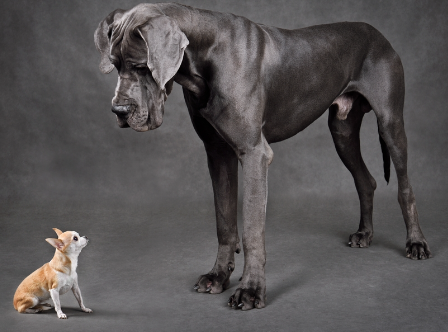
\includegraphics[width=.15\textwidth]{ModelDevelopment} \textit{Should we add an instruction where the drain elevation is specified?  }

A recharge boundary condition forces  water to flow in to the \gwf\ model domain at a specified rate.   To add a recharge  to the \gwf\ model domain use this instruction:

\ins{gwf recharge}
    {
        \squish
        \begin{enumerate}
            \item \rnum{value}  Recharge rate [L/T].
            \item \inum{option}  Recharge option.
        \end{enumerate}
        A recharge rate of \rnum{value} is assigned to the chosen cells.

        The recharge option \inum{option}is used to define where the recharge  is to be applied and can have one of the following values:
        \begin{enumerate}
            \item To top layer
            \item To one specified node in each vertical column
            \item To highest active node in each vertical column
            \item To the swf domain on top of each vertical column
        \end{enumerate}
        \squish
    }

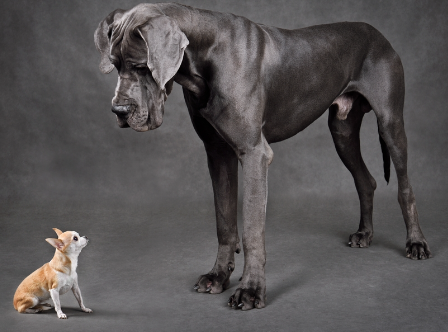
\includegraphics[width=.15\textwidth]{ModelDevelopment} \textit{Sould we have an example of pumping with an assigned nodal flux?  Should it be from a CLN?  Is there a boundary condition that assures the head will not be drawn down below the pumping node elevation?}





